\section{考察}
表\ref{tbl:応力値と信頼限界}より,塑性変形前の残留応力はA点,B点のどちらも圧縮応力を示した.塑性変形後の残留応力はA点ではやや値が下がったものの圧縮のままであったが,B点では引張応力に変化した.

これは塑性変形による応力分布と弾性変形による応力分布の差によって生じたものと考えられる.図\ref{fig:応力分布}に曲げ時の応力と除荷後の残留応力の分布を示す.(b)におけるAOA'が曲げ加工時の塑性変形によるものであり,BOB'が弾性変形によるものである.曲げ加工時,材料表面において塑性変形による応力が弾性変形によるものよりも小さくなっていることが分かる.荷重を除去すると,スプリングバックが生じて,弾性変形の分の応力が除去されることで(c)のような塑性変形による残留応力が残る.このような塑性変形による非線形な応力分布の結果,曲げ加工の外側であるA点では圧縮応力が残留し,内側であるB点では引張応力が残留したと考えることができる.

塑性変形後のA点において圧縮応力がやや下がった原因としては,曲げ加工時の引張応力による組織の変化によって,元々の圧縮応力が部分的に除去されたことが考えられる.
\clearpage
\begin{figure}[htbp]
    \centering %中央揃え
    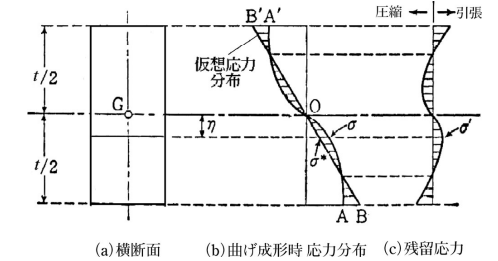
\includegraphics[width=100truemm,clip]{fig/応力分布.png}
    \caption{Stress in bending and residual stress after unloading.\cite{応力分布}}
    \label{fig:応力分布}
\end{figure}
% これは材料内部の反発によるものであると考えられる.つまり,外側であるA点では加工時に引張応力が加わるため,反発として圧縮応力が残留し,一方内側であるB点では加工時に圧縮応力が加わるため,反発として引張応力が残留したということである.



